\documentclass[12pt, letterpaper, twoside]{article}\usepackage[]{graphicx}\usepackage[]{xcolor}
% maxwidth is the original width if it is less than linewidth
% otherwise use linewidth (to make sure the graphics do not exceed the margin)
\makeatletter
\def\maxwidth{ %
  \ifdim\Gin@nat@width>\linewidth
    \linewidth
  \else
    \Gin@nat@width
  \fi
}
\makeatother

\definecolor{fgcolor}{rgb}{0.345, 0.345, 0.345}
\newcommand{\hlnum}[1]{\textcolor[rgb]{0.686,0.059,0.569}{#1}}%
\newcommand{\hlstr}[1]{\textcolor[rgb]{0.192,0.494,0.8}{#1}}%
\newcommand{\hlcom}[1]{\textcolor[rgb]{0.678,0.584,0.686}{\textit{#1}}}%
\newcommand{\hlopt}[1]{\textcolor[rgb]{0,0,0}{#1}}%
\newcommand{\hlstd}[1]{\textcolor[rgb]{0.345,0.345,0.345}{#1}}%
\newcommand{\hlkwa}[1]{\textcolor[rgb]{0.161,0.373,0.58}{\textbf{#1}}}%
\newcommand{\hlkwb}[1]{\textcolor[rgb]{0.69,0.353,0.396}{#1}}%
\newcommand{\hlkwc}[1]{\textcolor[rgb]{0.333,0.667,0.333}{#1}}%
\newcommand{\hlkwd}[1]{\textcolor[rgb]{0.737,0.353,0.396}{\textbf{#1}}}%
\let\hlipl\hlkwb

\usepackage{framed}
\makeatletter
\newenvironment{kframe}{%
 \def\at@end@of@kframe{}%
 \ifinner\ifhmode%
  \def\at@end@of@kframe{\end{minipage}}%
  \begin{minipage}{\columnwidth}%
 \fi\fi%
 \def\FrameCommand##1{\hskip\@totalleftmargin \hskip-\fboxsep
 \colorbox{shadecolor}{##1}\hskip-\fboxsep
     % There is no \\@totalrightmargin, so:
     \hskip-\linewidth \hskip-\@totalleftmargin \hskip\columnwidth}%
 \MakeFramed {\advance\hsize-\width
   \@totalleftmargin\z@ \linewidth\hsize
   \@setminipage}}%
 {\par\unskip\endMakeFramed%
 \at@end@of@kframe}
\makeatother

\definecolor{shadecolor}{rgb}{.97, .97, .97}
\definecolor{messagecolor}{rgb}{0, 0, 0}
\definecolor{warningcolor}{rgb}{1, 0, 1}
\definecolor{errorcolor}{rgb}{1, 0, 0}
\newenvironment{knitrout}{}{} % an empty environment to be redefined in TeX

\usepackage{alltt}

\usepackage{amsmath}
\usepackage{booktabs}
\usepackage{amsthm}
\usepackage{lipsum}
\usepackage{graphicx}
\usepackage[margin=1in]{geometry}
\usepackage[colorlinks=true]{hyperref}
\hypersetup{colorlinks = true, linkcolor = blue, citecolor=blue, urlcolor = blue}
\usepackage{natbib}
\usepackage{enumitem}
\usepackage{setspace}
\graphicspath{ {/Users/patrickbrogan/Desktop/R/} }

\usepackage[pagewise]{lineno}
%\linenumbers*[1]
% %% patches to make lineno work better with amsmath
\newcommand*\patchAmsMathEnvironmentForLineno[1]{%
 \expandafter\let\csname old#1\expandafter\endcsname\csname #1\endcsname
 \expandafter\let\csname oldend#1\expandafter\endcsname\csname end#1\endcsname
 \renewenvironment{#1}%
 {\linenomath\csname old#1\endcsname}%
 {\csname oldend#1\endcsname\endlinenomath}}%
\newcommand*\patchBothAmsMathEnvironmentsForLineno[1]{%
 \patchAmsMathEnvironmentForLineno{#1}%
 \patchAmsMathEnvironmentForLineno{#1*}}%

 \AtBeginDocument{%
 \patchBothAmsMathEnvironmentsForLineno{equation}%
 \patchBothAmsMathEnvironmentsForLineno{align}%
 \patchBothAmsMathEnvironmentsForLineno{flalign}%
 \patchBothAmsMathEnvironmentsForLineno{alignat}%
 \patchBothAmsMathEnvironmentsForLineno{gather}%
 \patchBothAmsMathEnvironmentsForLineno{multline}%
}

\title{STAT 3494W Paper}
\author{Patrick Brogan\\[1ex]
  Department of Statistics, University of Connecticut\\}
\date{September 2022}
\IfFileExists{upquote.sty}{\usepackage{upquote}}{}
\begin{document}

\maketitle

\begin{abstract}
\lipsum[3]
\end{abstract}

\section*{Introduction}
\addcontentsline{toc}{section}{Introduction}
Here is a link to \href{http://www.overleaf.com}{Overleaf}. \lipsum[5]
\section*{Methods}
\addcontentsline{toc}{section}{Methods}
What did you do? – a section which details how the research was
performed.  It typically features a description of the participants/
subjects that were involved, the study design, the materials that were
used, and the study procedure.  If there were multiple experiments,
then each experiment may require a separate Methods section.  A rule
of thumb is that the Methods section should be sufficiently detailed
for another researcher to duplicate your research. Inline equations should look like \(e^{i\theta} = \cos(\theta) + i\sin\theta\). Use displaystyle equations like so \begin{equation}
  f(y) = \frac{1}{\Gamma(\alpha)\beta^\alpha}\*y^{\alpha-1}e^{-\frac{y}{\beta}}, y > 0,
\end{equation}
Equations without numbers should look like this
\[
  E[Y] = \int_{-\infty}^{\infty} yf(y) \,dy,
\]


\section*{Results}
\addcontentsline{toc}{section}{Results}
\lipsum[6]

\begin{center}
\begin{tabular}{||c c c c||}
 \hline
 Uniform & Exponential & Normal & Gamma \\ [0.5ex]
 \hline\hline
 0.3752854 & 0.8941359 & 1.0891278 & 1.8365839 \\
 \hline
 0.3429779 & 1.5657469 & 0.6783542 & 0.2391189 \\
 \hline
 0.5412031 & 2.0190394 & -0.2033725 & 1.0632763 \\
 \hline
 0.0224390 & 1.2995342 & 0.2241231 & 0.2357952 \\
 \hline
 0.4368829 & 0.2267861 & -0.3625344 & 3.3227355 \\ [1ex]
 \hline
\end{tabular}
\end{center}

\begin{figure}[h]
  \centering
  \caption{Table of random numbers generated from different probability distributions}
  \label{fig:Random Variable Table}
\end{figure}

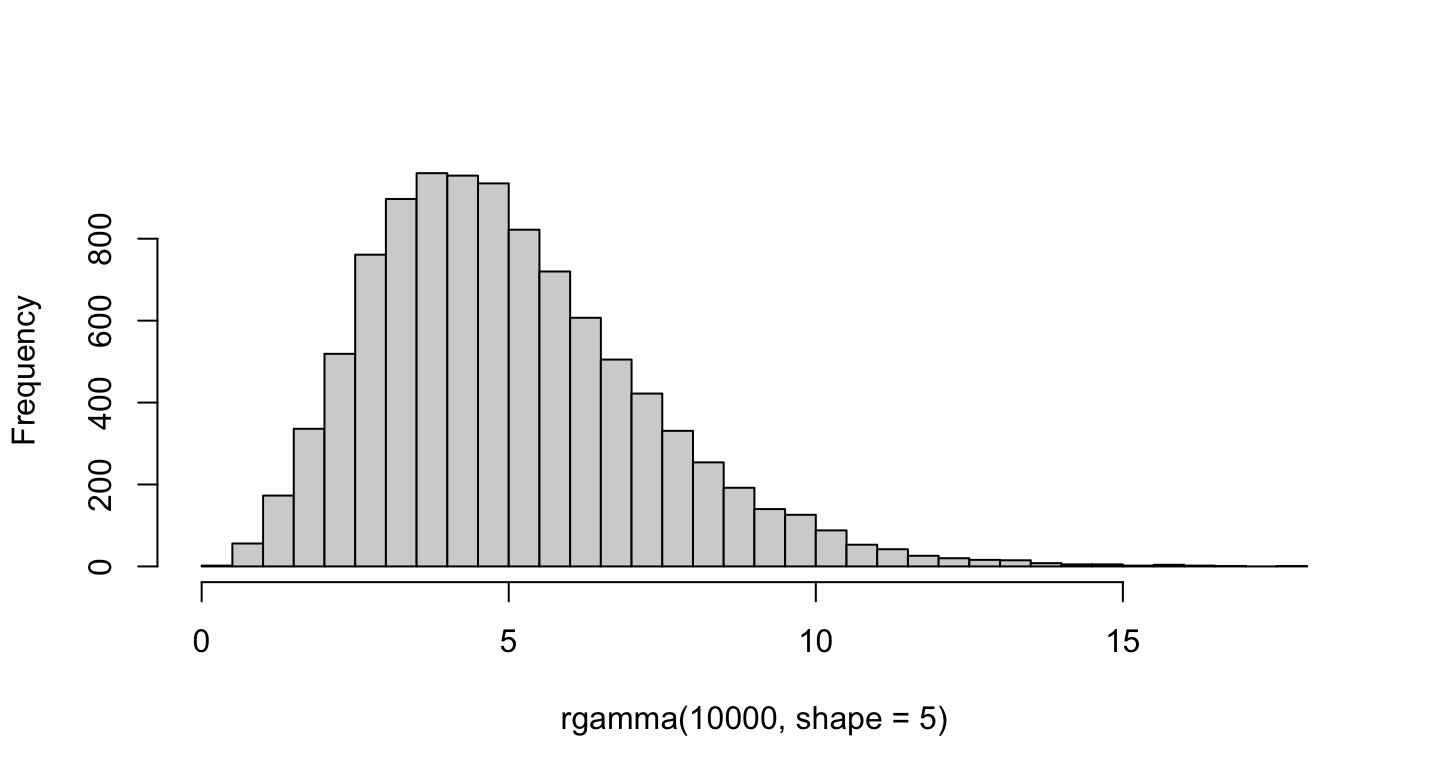
\includegraphics[scale=0.7]{GammaHist.pdf}

\begin{figure}[h]
  \centering
  \caption{Histogram of randomly generated numbers from a gamma probability distribution}
  \label{fig:Random Gamma Histogram}
\end{figure}

\section*{Discussion}
\lipsum[-1]

\section*{References}
\lipsum[7]

\end{document}

